\KOMAoptions{paper=A3}
\recalctypearea
\subsection{Modular Times Table}{\label{pp:timestable}}
Procedure to construct the Modular Times Table:
\begin{itemize}
	\item Draw a circle which fits the entire ``drawing canvas''.
	\item Imagine you have $n$ equally-spaced points on the circumference of this circle. Number them $0$ to $n-1$ anti-clockwise with $0$ being the leftmost point.
	\item For each $i \in \{0,1,2,\ldots,n-1\}$ connect the points representing $i$ with the point for $(m\cdot i)\ \%\ n$ with a straight line.
\end{itemize} An example is shown in \ref{fig:timestable}. Don't draw the numbers. They are just to visualise the construction.
\begin{figure}[H]
	\centering
	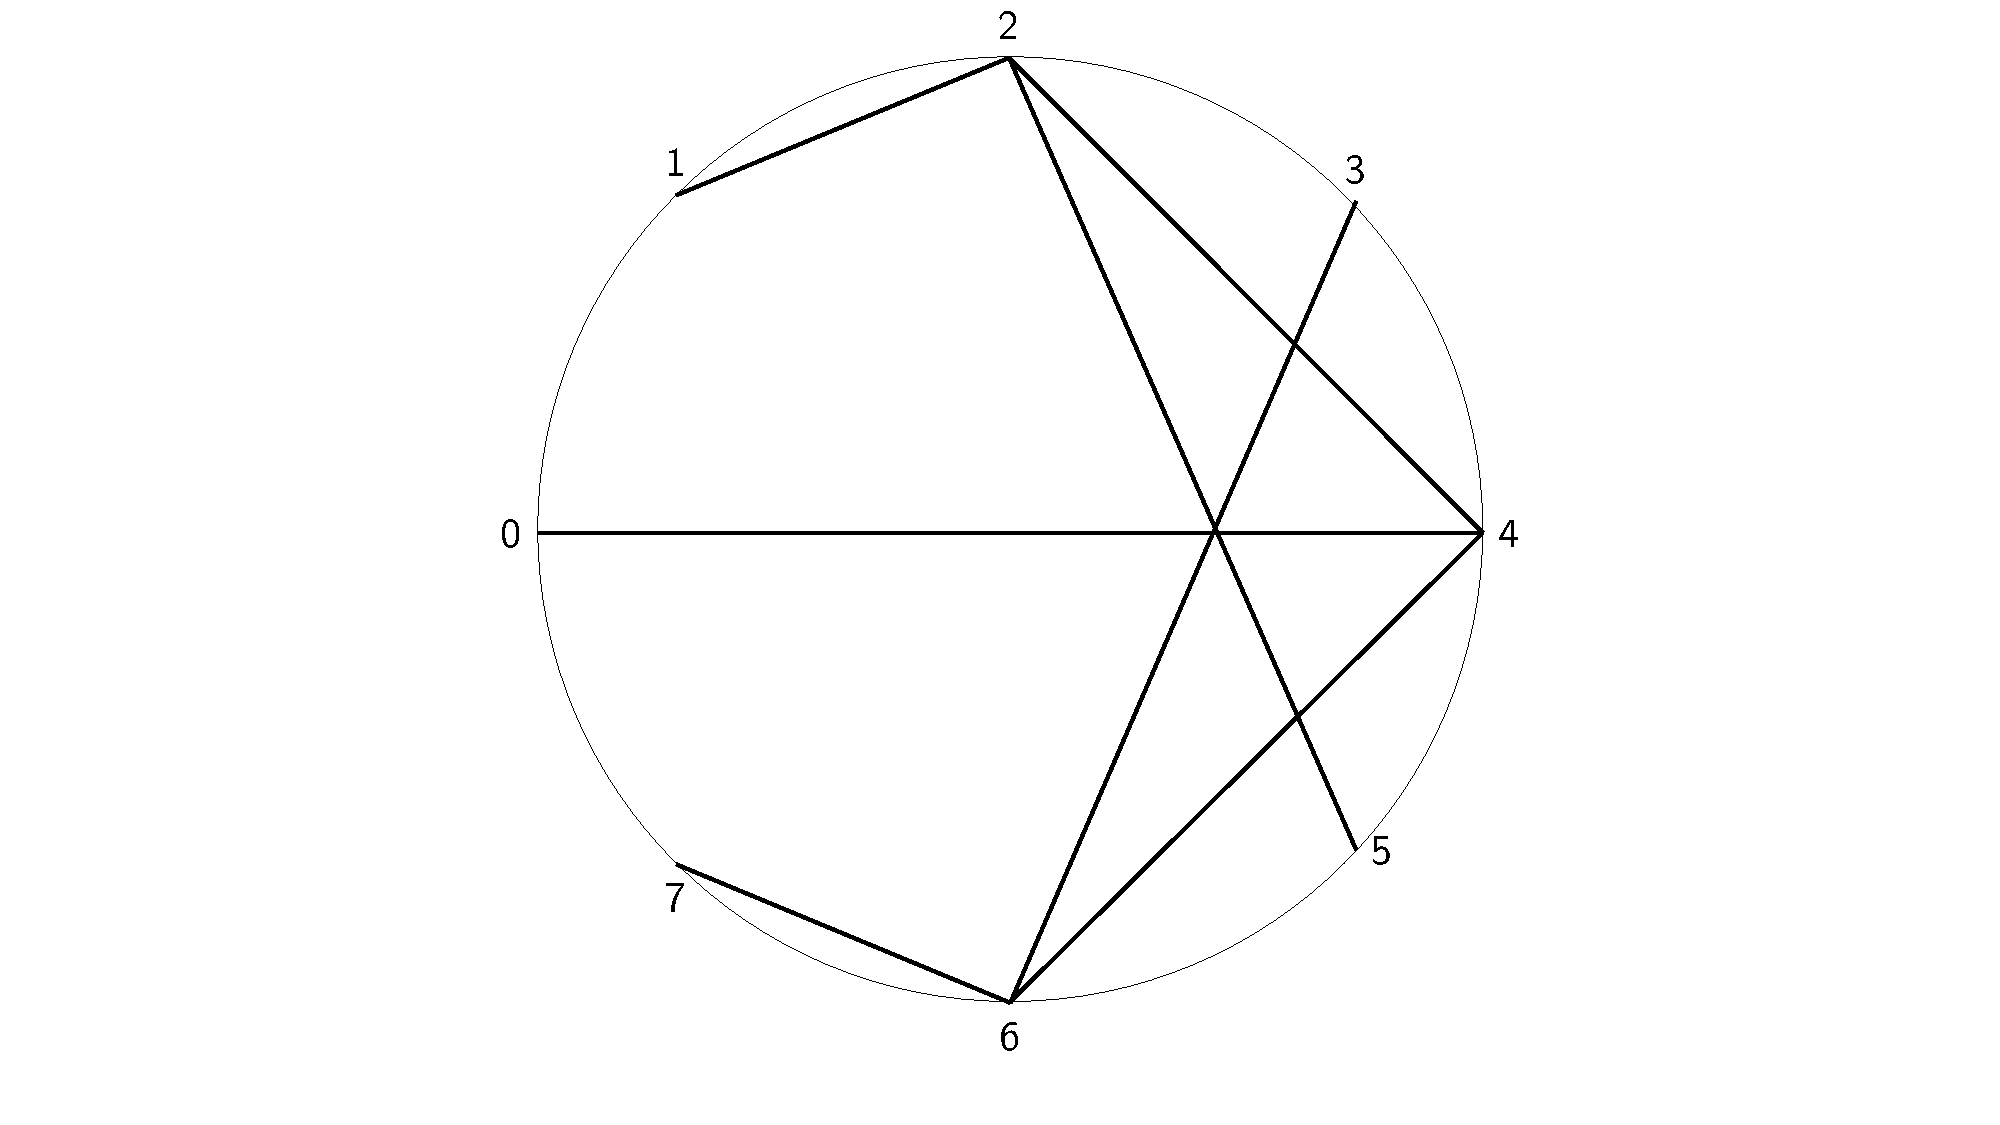
\includegraphics[width = 0.18\linewidth]{Modular Times Table.pdf}
	\caption{Times Table for $(n,m)=(8,2)$}
	\label{fig:timestable}
\end{figure}
\textbf{Problem Statement:}\\
For a given $(n,m)$ pair $(n>m)$, construct the Modular Times Table.
\begin{testcases}
	{$n\quad m$ \hfill(two numbers)}
	{The constructed Modular Times Table}
	{$3 \leq n \leq 500$\hfill(an integer)\\
	$1 < m < n$ \hfill(a double, first try to solve the problem for an integer $m$)}
	{See \ref{fig:timestabletestcases}}
	{See \ref{fig:timestabletestcases}}
	{https://github.com/paramrathour/CS-101/tree/main/Starter Codes/Modular Times Table.cpp}
\end{testcases}
\textbf{The output Modular Times Tables}
\begin{figure}[H]
	\centering
	\begin{subfigure}{0.145\linewidth}
		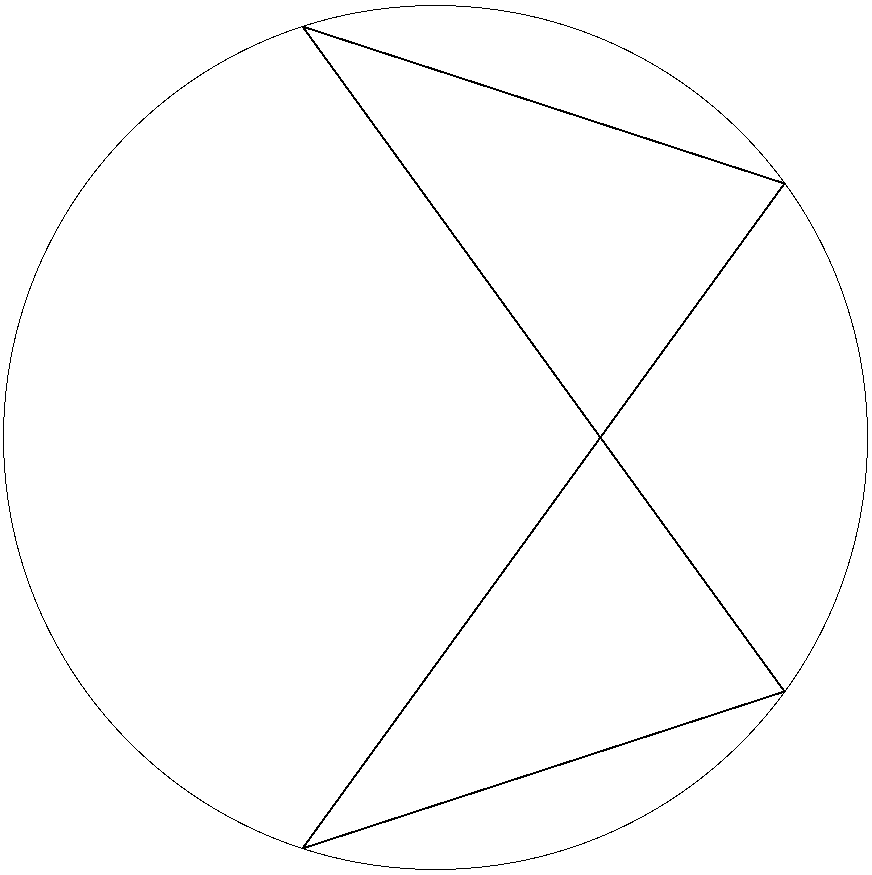
\includegraphics[width = \linewidth]{Modular Times Table/5 2.png}
		\caption{$(n,m) = (5,2)$}
	\end{subfigure}
	\begin{subfigure}{0.145\linewidth}
		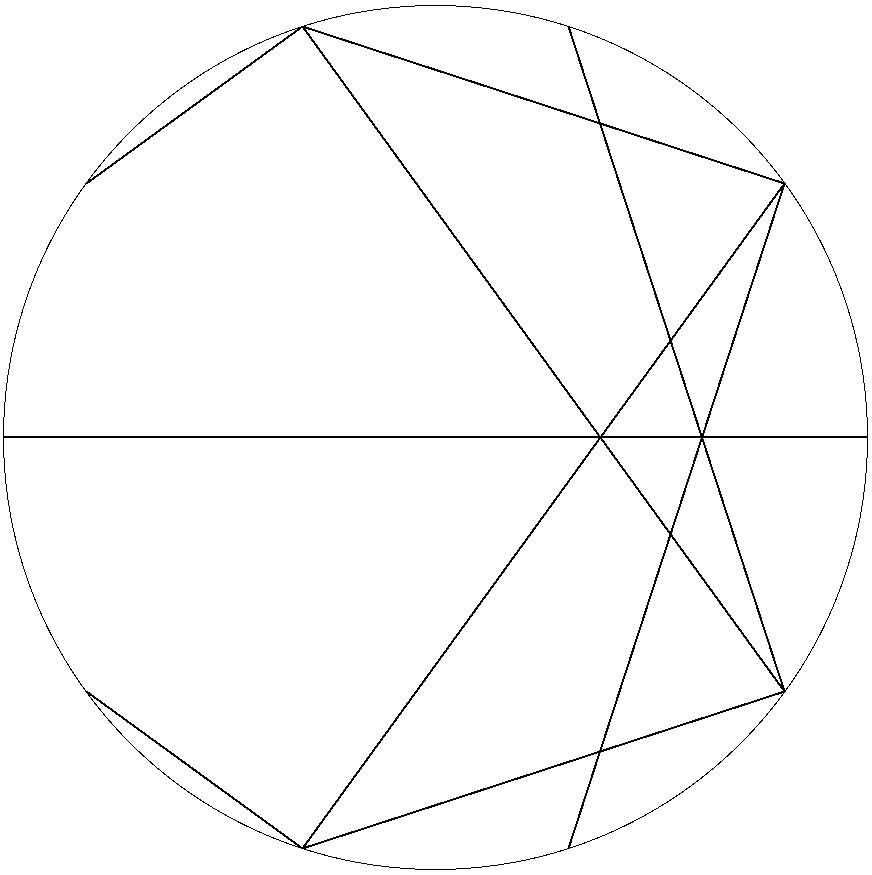
\includegraphics[width = \linewidth]{Modular Times Table/10 2.png}
		\caption{$(n,m) = (10,2)$}
	\end{subfigure}
	\begin{subfigure}{0.145\linewidth}
		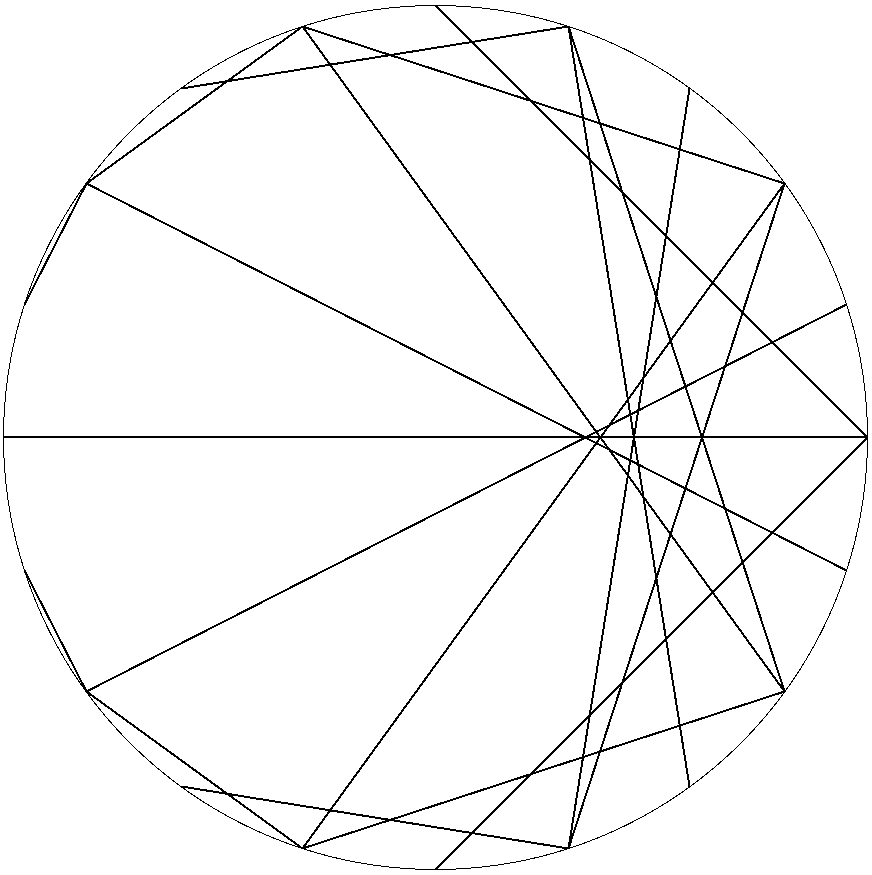
\includegraphics[width = \linewidth]{Modular Times Table/20 2.png}
		\caption{$(n,m) = (20,2)$}
	\end{subfigure}
	\begin{subfigure}{0.145\linewidth}
		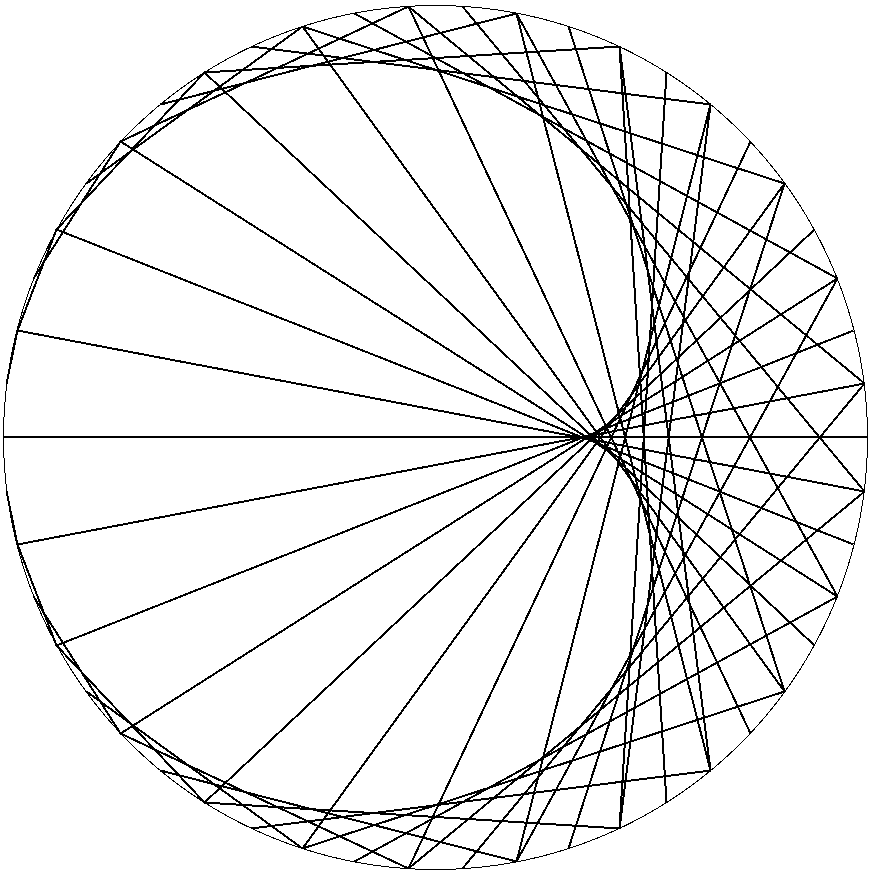
\includegraphics[width = \linewidth]{Modular Times Table/50 2.png}
		\caption{$(n,m) = (50,2)$}
	\end{subfigure}
	\begin{subfigure}{0.145\linewidth}
		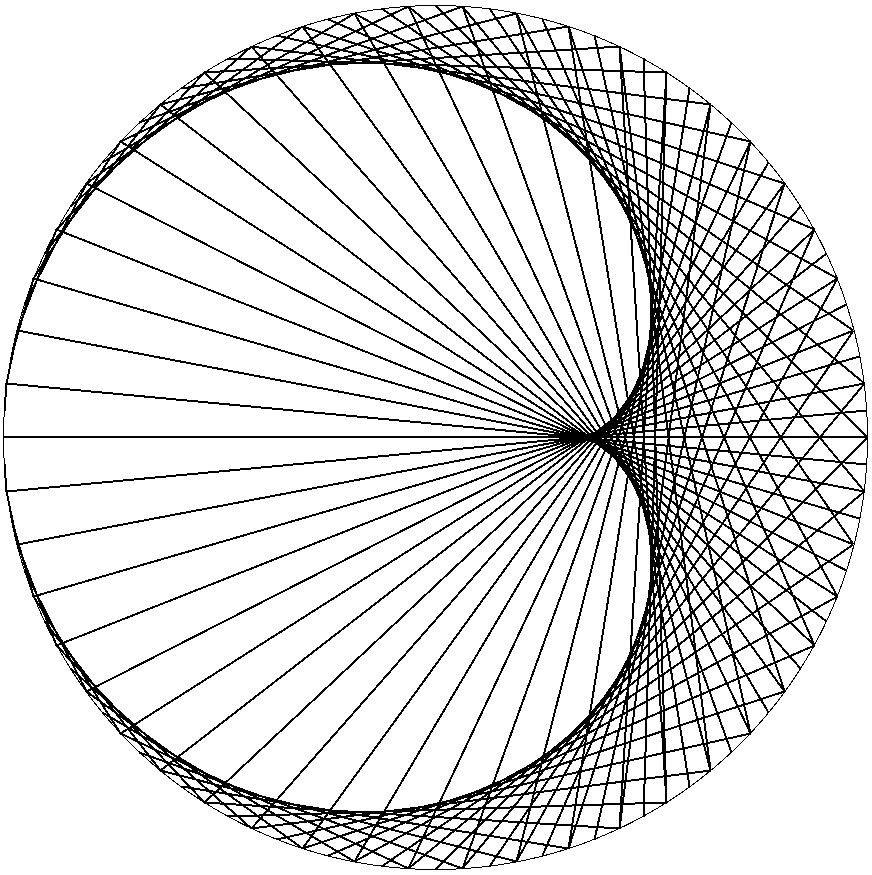
\includegraphics[width = \linewidth]{Modular Times Table/100 2.png}
		\caption{$(n,m) = (100,2)$}
	\end{subfigure}
	\begin{subfigure}{0.145\linewidth}
		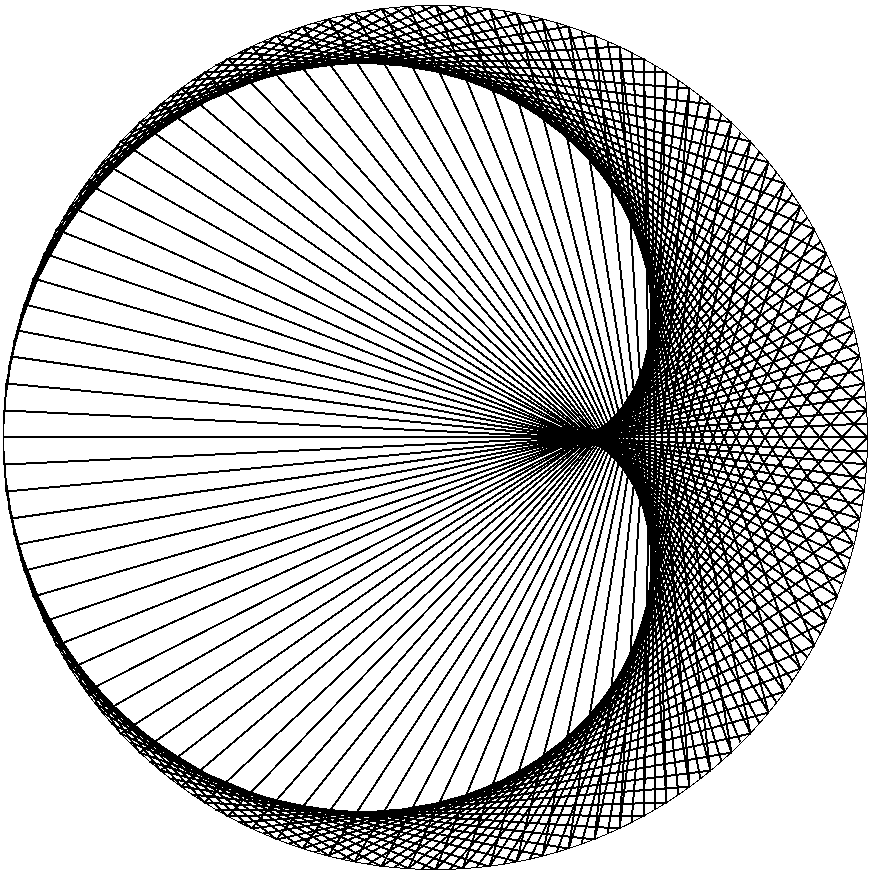
\includegraphics[width = \linewidth]{Modular Times Table/200 2.png}
		\caption{$(n,m) = (200,2)$}
	\end{subfigure}
		\begin{subfigure}{0.145\linewidth}
		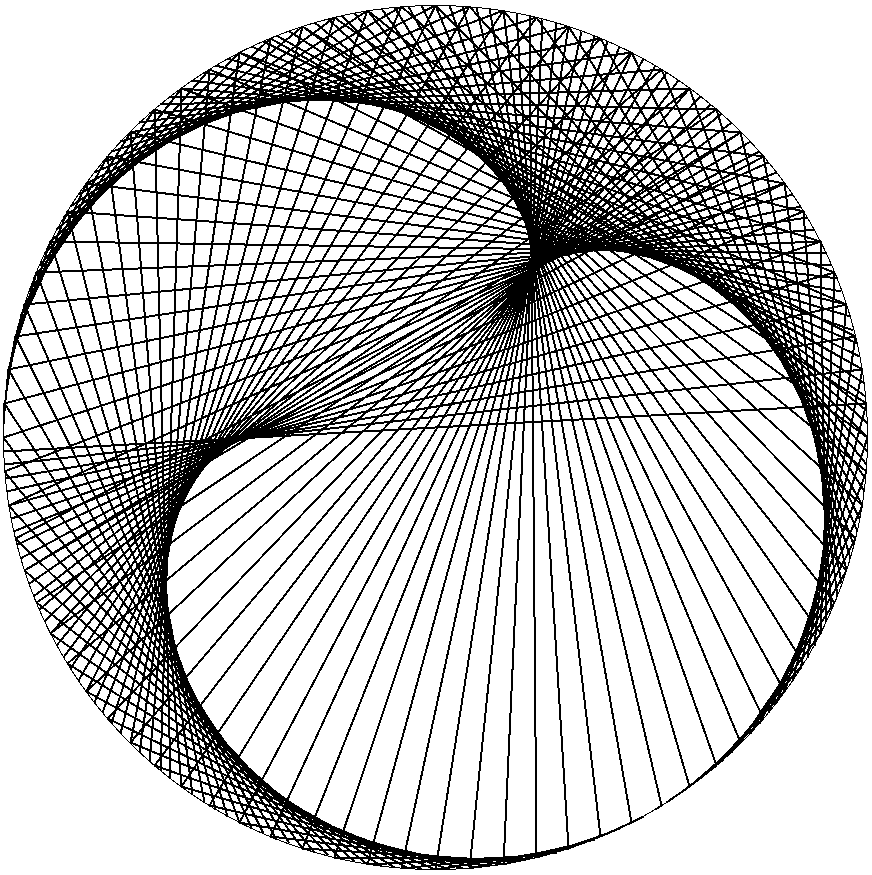
\includegraphics[width = \linewidth]{Modular Times Table/200 2.5.png}
		\caption{$(n,m) = (200,2.5)$}
	\end{subfigure}
	\begin{subfigure}{0.145\linewidth}
		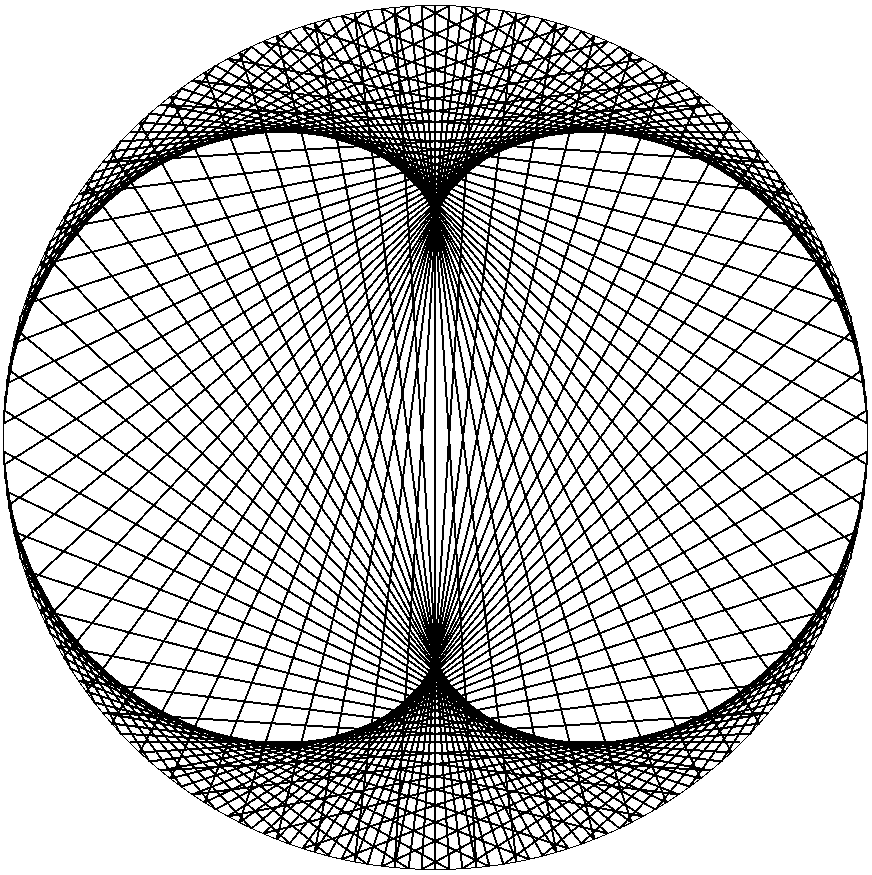
\includegraphics[width = \linewidth]{Modular Times Table/200 3.png}
		\caption{$(n,m) = (200,3)$}
	\end{subfigure}
	\begin{subfigure}{0.145\linewidth}
		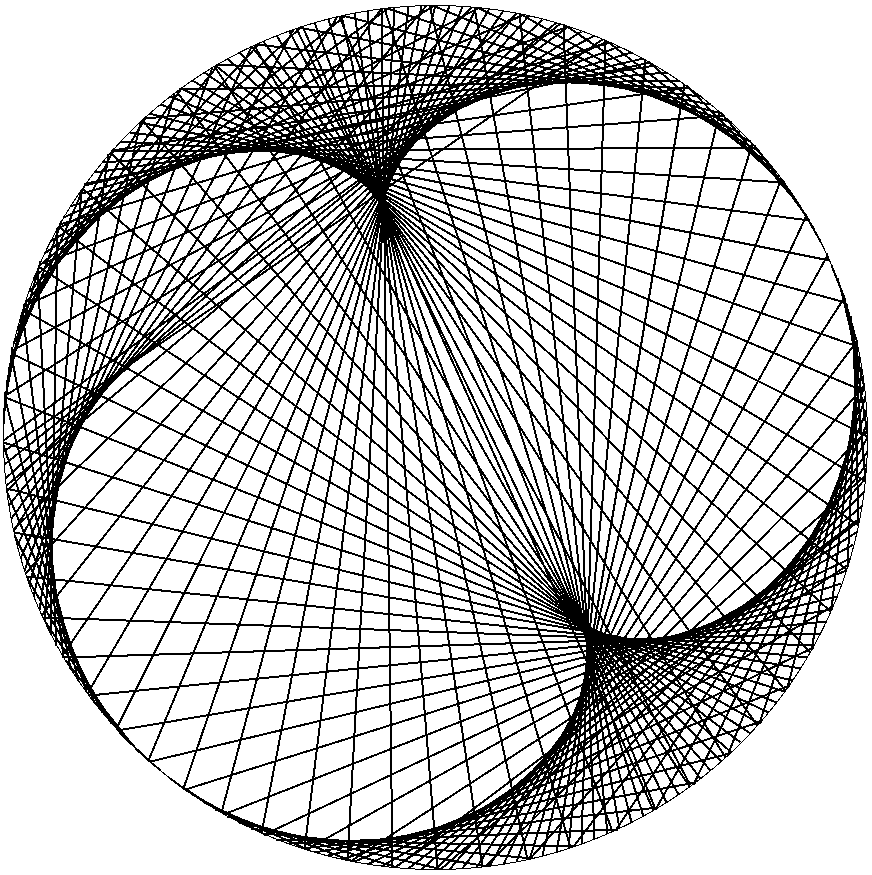
\includegraphics[width = \linewidth]{Modular Times Table/200 3.33.png}
		\caption{$(n,m) = (200,3.33)$}
	\end{subfigure}
	\begin{subfigure}{0.145\linewidth}
		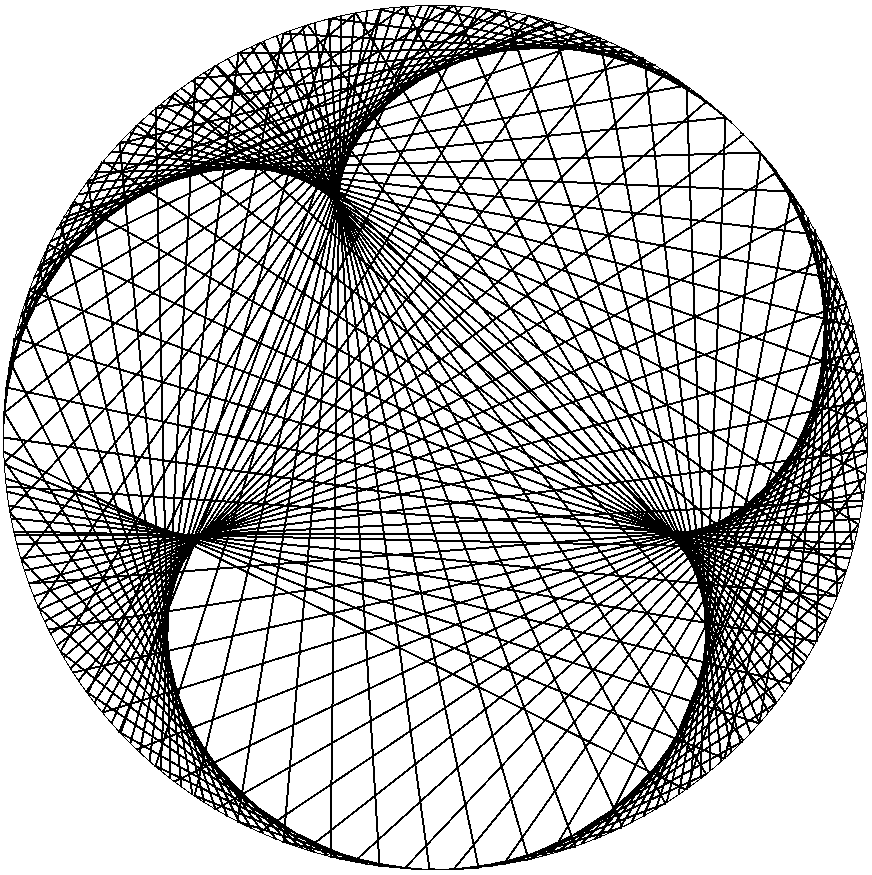
\includegraphics[width = \linewidth]{Modular Times Table/200 3.66.png}
		\caption{$(n,m) = (200,3.66)$}
	\end{subfigure}
	\begin{subfigure}{0.145\linewidth}
		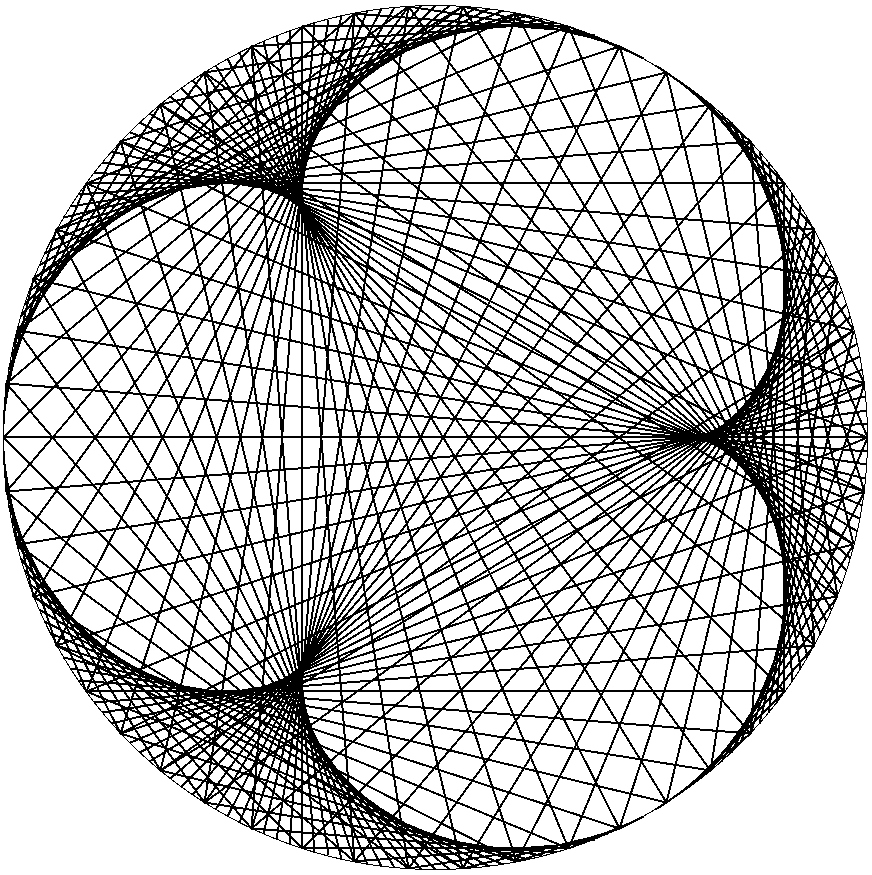
\includegraphics[width = \linewidth]{Modular Times Table/200 4.png}
		\caption{$(n,m) = (200,4)$}
	\end{subfigure}
	\begin{subfigure}{0.145\linewidth}
		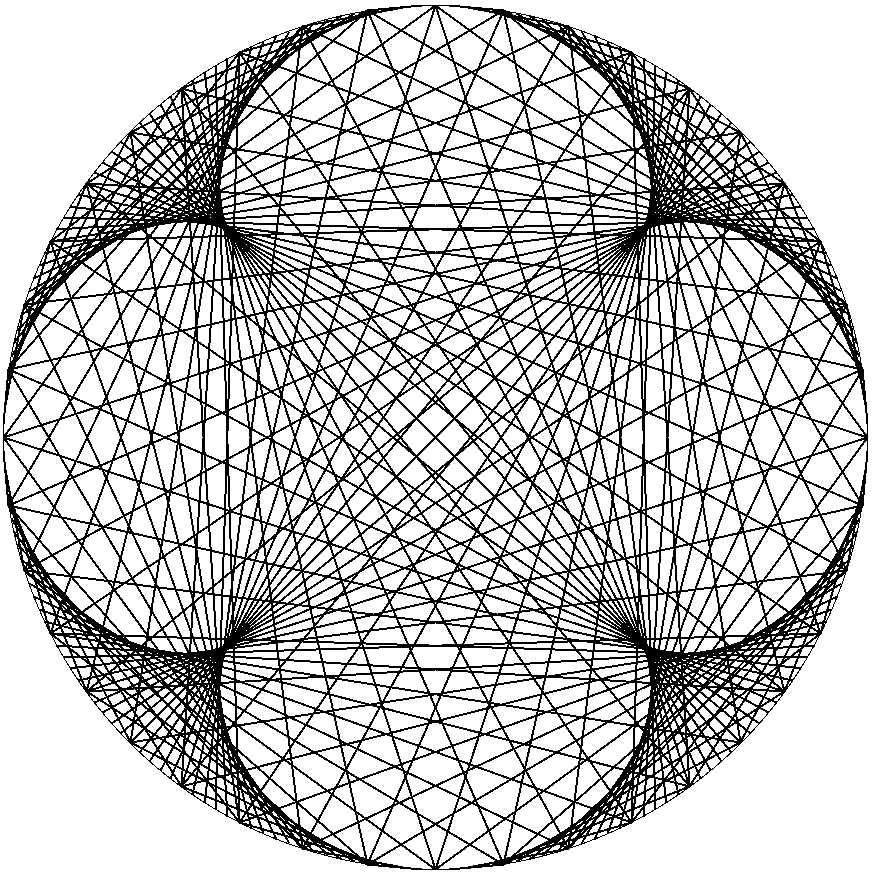
\includegraphics[width = \linewidth]{Modular Times Table/200 5.png}
		\caption{$(n,m) = (200,5)$}
	\end{subfigure}
	\begin{subfigure}{0.145\linewidth}
		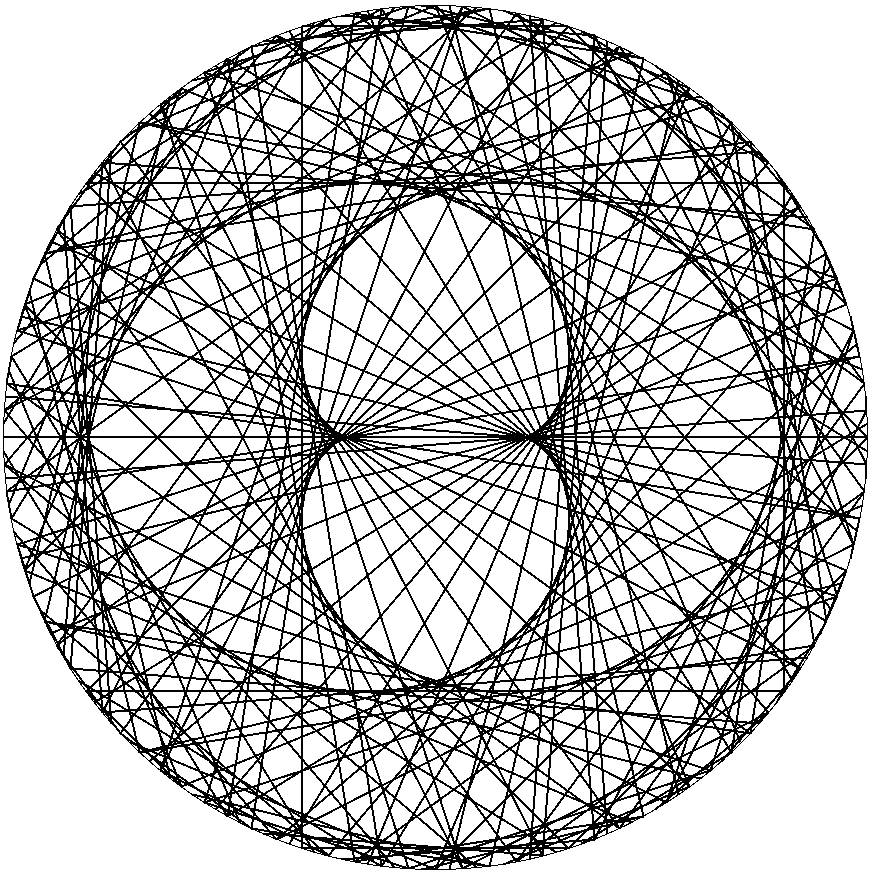
\includegraphics[width = \linewidth]{Modular Times Table/200 34.png}
		\caption{$(n,m) = (200,34)$}
	\end{subfigure}
	\begin{subfigure}{0.145\linewidth}
		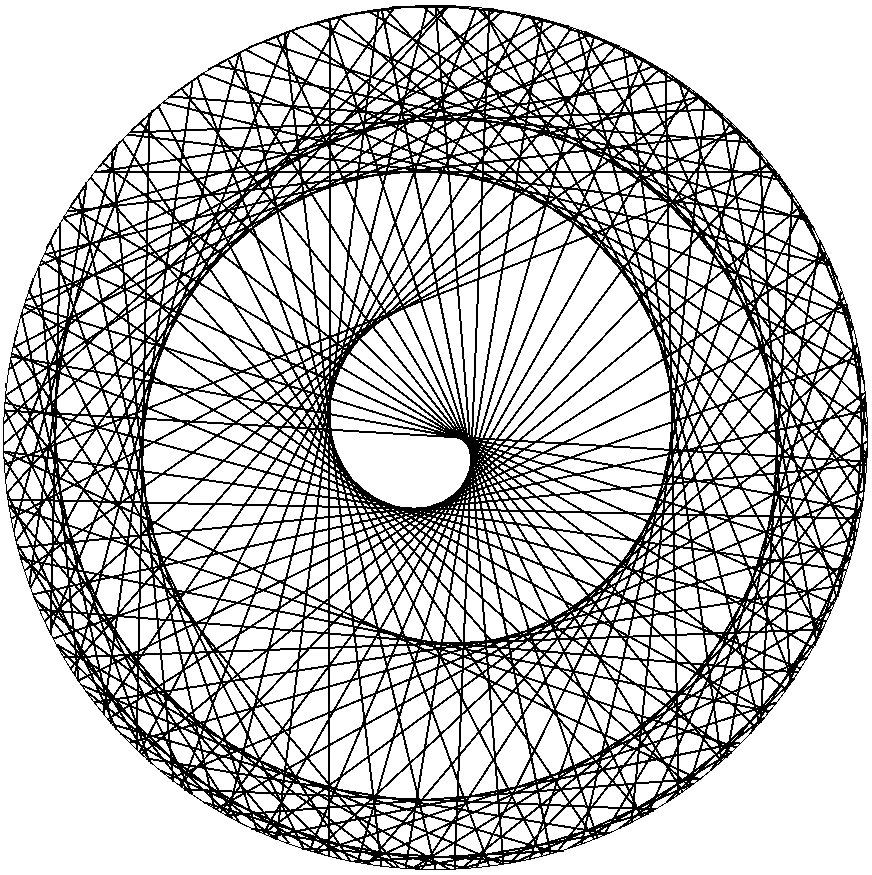
\includegraphics[width = \linewidth]{Modular Times Table/200 50.9.png}
		\caption{$(n,m) = (200,50.9)$}
	\end{subfigure}
	\begin{subfigure}{0.145\linewidth}
		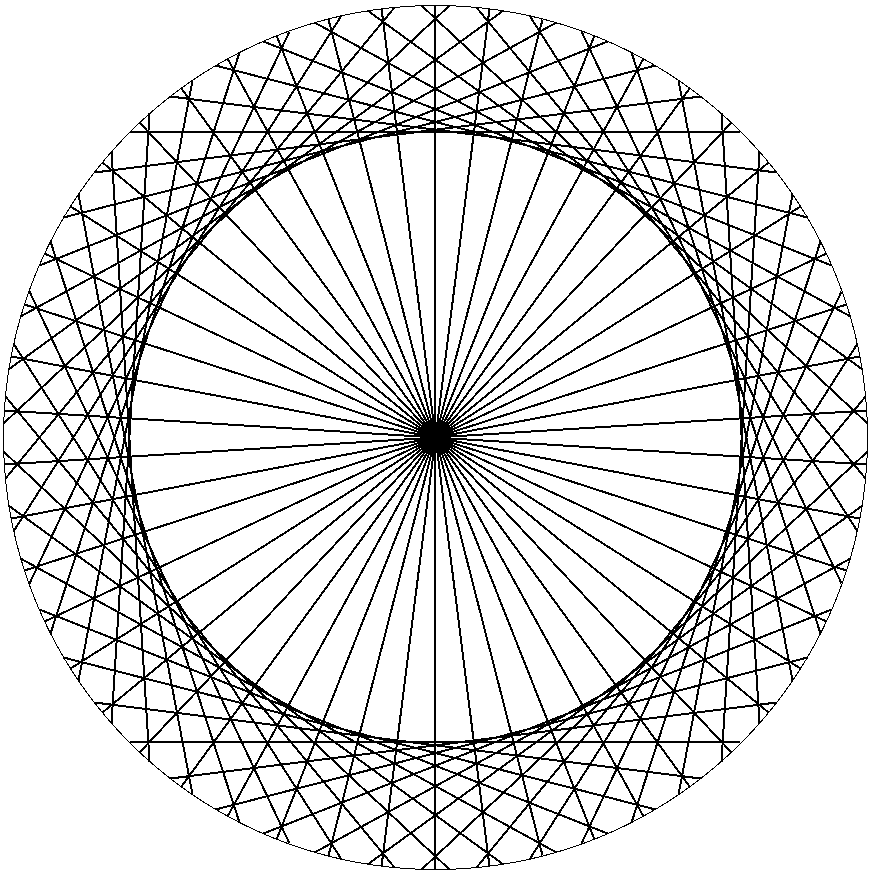
\includegraphics[width = \linewidth]{Modular Times Table/200 51.png}
		\caption{$(n,m) = (200,51)$}
	\end{subfigure}
	\begin{subfigure}{0.145\linewidth}
		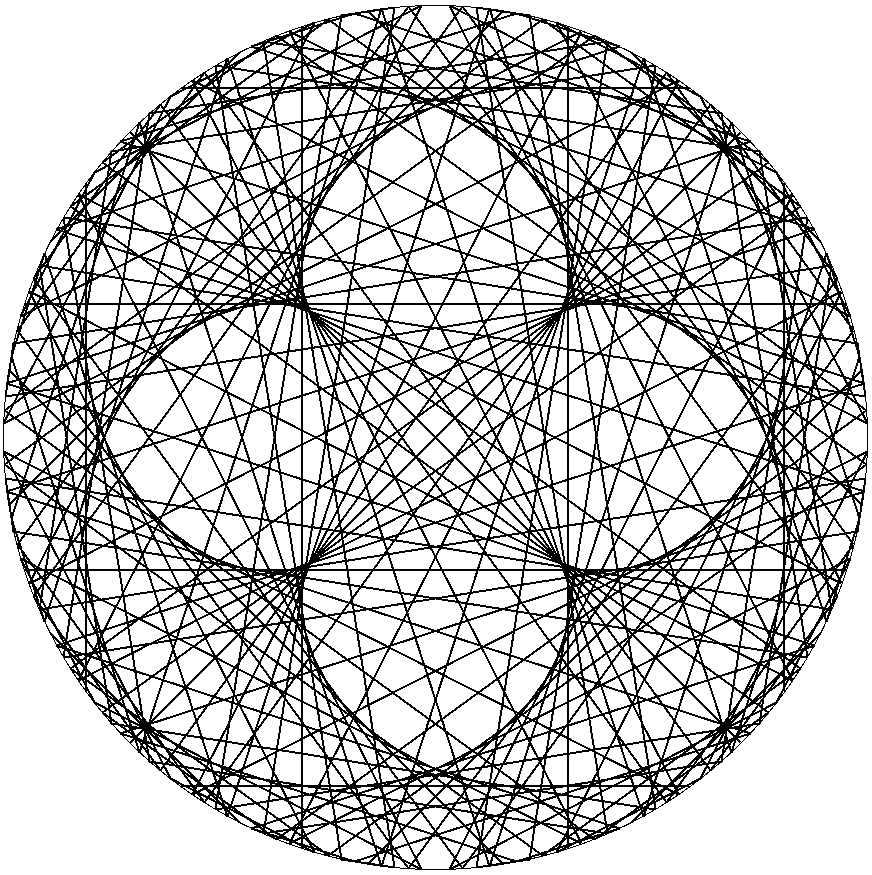
\includegraphics[width = \linewidth]{Modular Times Table/200 69.png}
		\caption{$(n,m) = (200,69)$}
	\end{subfigure}
	\begin{subfigure}{0.145\linewidth}
		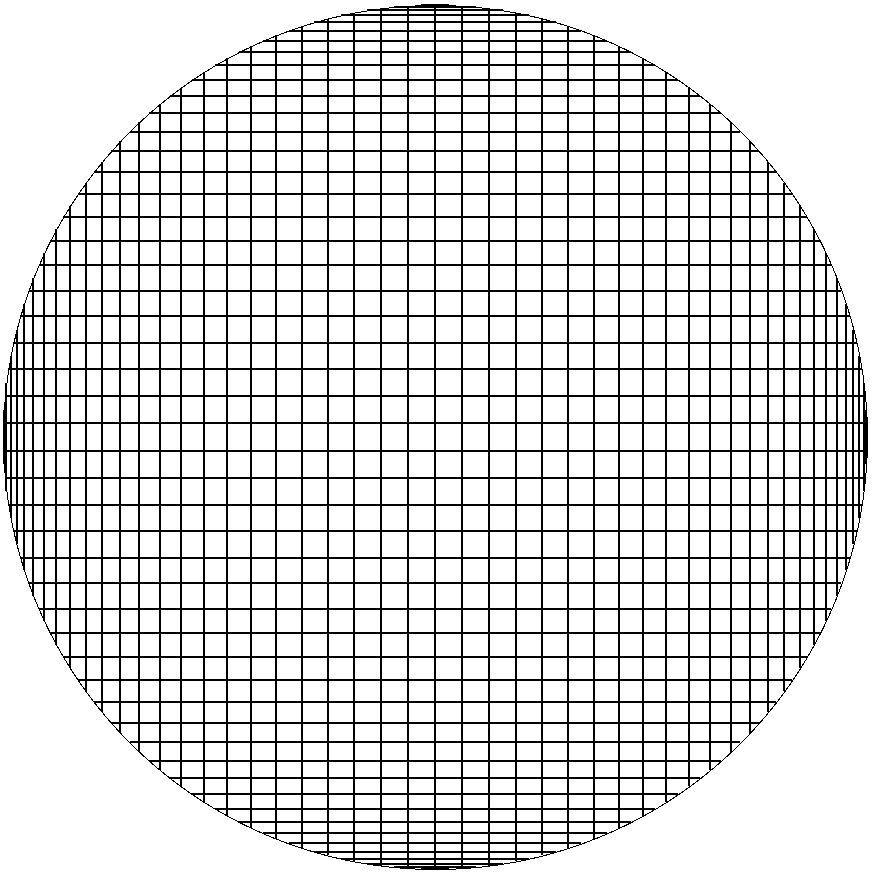
\includegraphics[width = \linewidth]{Modular Times Table/200 99.png}
		\caption{$(n,m) = (200,99)$}
	\end{subfigure}
	\begin{subfigure}{0.145\linewidth}
		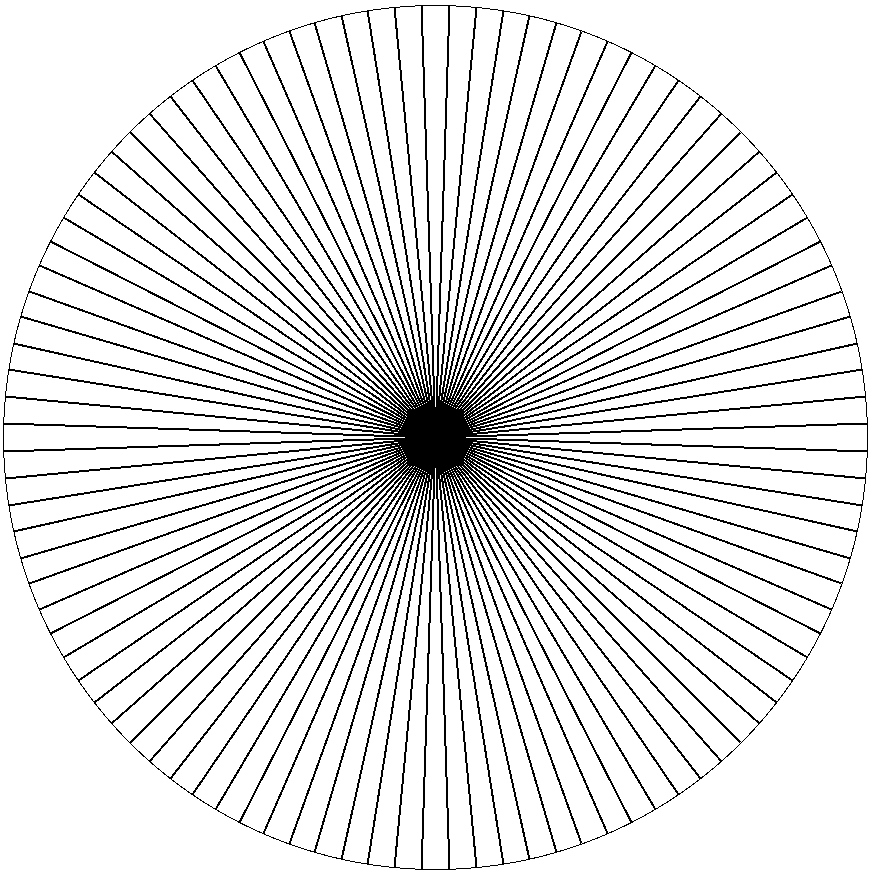
\includegraphics[width = \linewidth]{Modular Times Table/200 101.png}
		\caption{$(n,m) = (200,101)$}
	\end{subfigure}
	\caption{Modular Times Table}
	\label{fig:timestabletestcases}
\end{figure}
\begin{funvideo}
	\href{https://youtu.be/qhbuKbxJsk8}{Times Tables, Mandelbrot and the Heart of Mathematics}\\
	\href{https://www.geogebra.org/m/z8wrdret}{Modular Times Tables}
\end{funvideo}
\KOMAoptions{paper=A4}
\recalctypearea